\documentclass{beamer}

%\usepackage{pgfpages} % notes
%\setbeameroption{show notes on second screen=right} % notes
% for notes

\usepackage{Res/presento}
\setbeamercolor{background canvas}{bg=colorlgray}
\setbeamercolor{normal text}{fg=colorhgray}

%\usepackage{textpos}
%\setlength{\TPHorizModule}{1cm}
%\setlength{\TPVertModule}{1cm}
% for textblock

\usepackage{amsmath, amsfonts, amssymb}
\usepackage{graphicx, tikz}


\graphicspath{{Res/}}

\begin{document}
    \begin{frame}[plain]
        \vfill
        \largetext{
            \color{orange}{Dimitrije Glukčević  \\
            \setnote{dimchee90@gmail.com}}
        }
        \vfill
        \largetext{\color{colorblue}
            Da li je moguće smestiti Jokića u kutiju?
        }
        \setnote{Letnji seminar za mlađe polaznike, Petnica 2021}
        \vfill
        \scalebox{0.5}{\input{Res/pmf.pdf_tex}}
        \vfill
        \begin{tikzpicture}[remember picture,overlay]
            \node[anchor=north east] at (current page.north east) {
                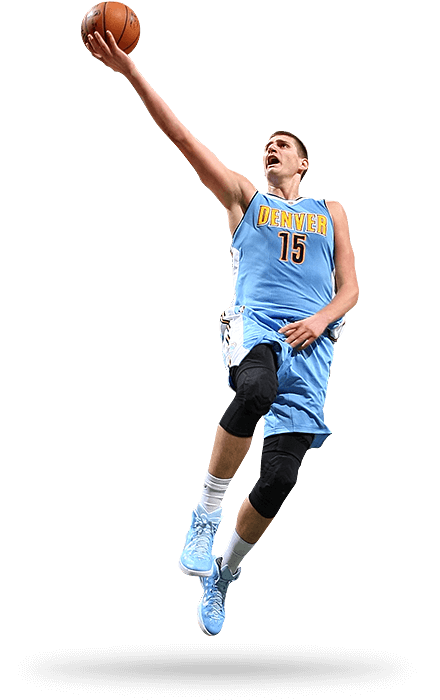
\includegraphics[height=0.8\textwidth]{Res/Jokic/Jokic_ceo}
            };
        \end{tikzpicture}
    \end{frame}

    \begin{frame}{Priče o superherojima}
        \note{test}
        .... Neke slike (i na kraju Jokić)
    \end{frame}
    \begin{frame}{}
        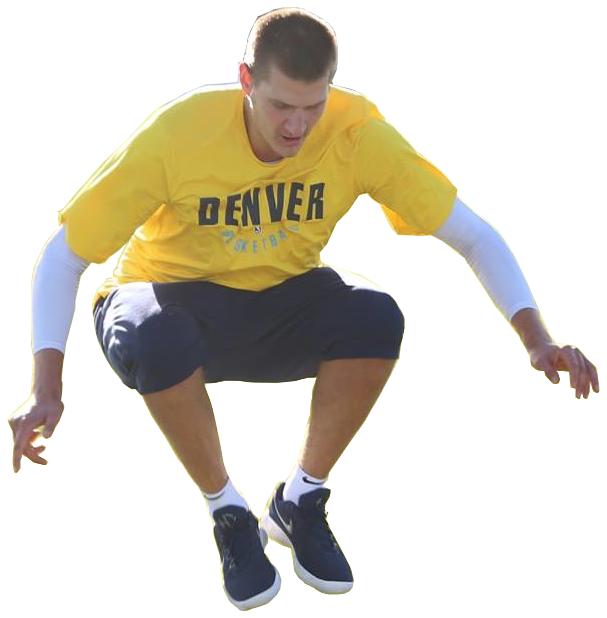
\includegraphics[height=0.4\textwidth]{Res/Jokic/Jokic_skok} \\
        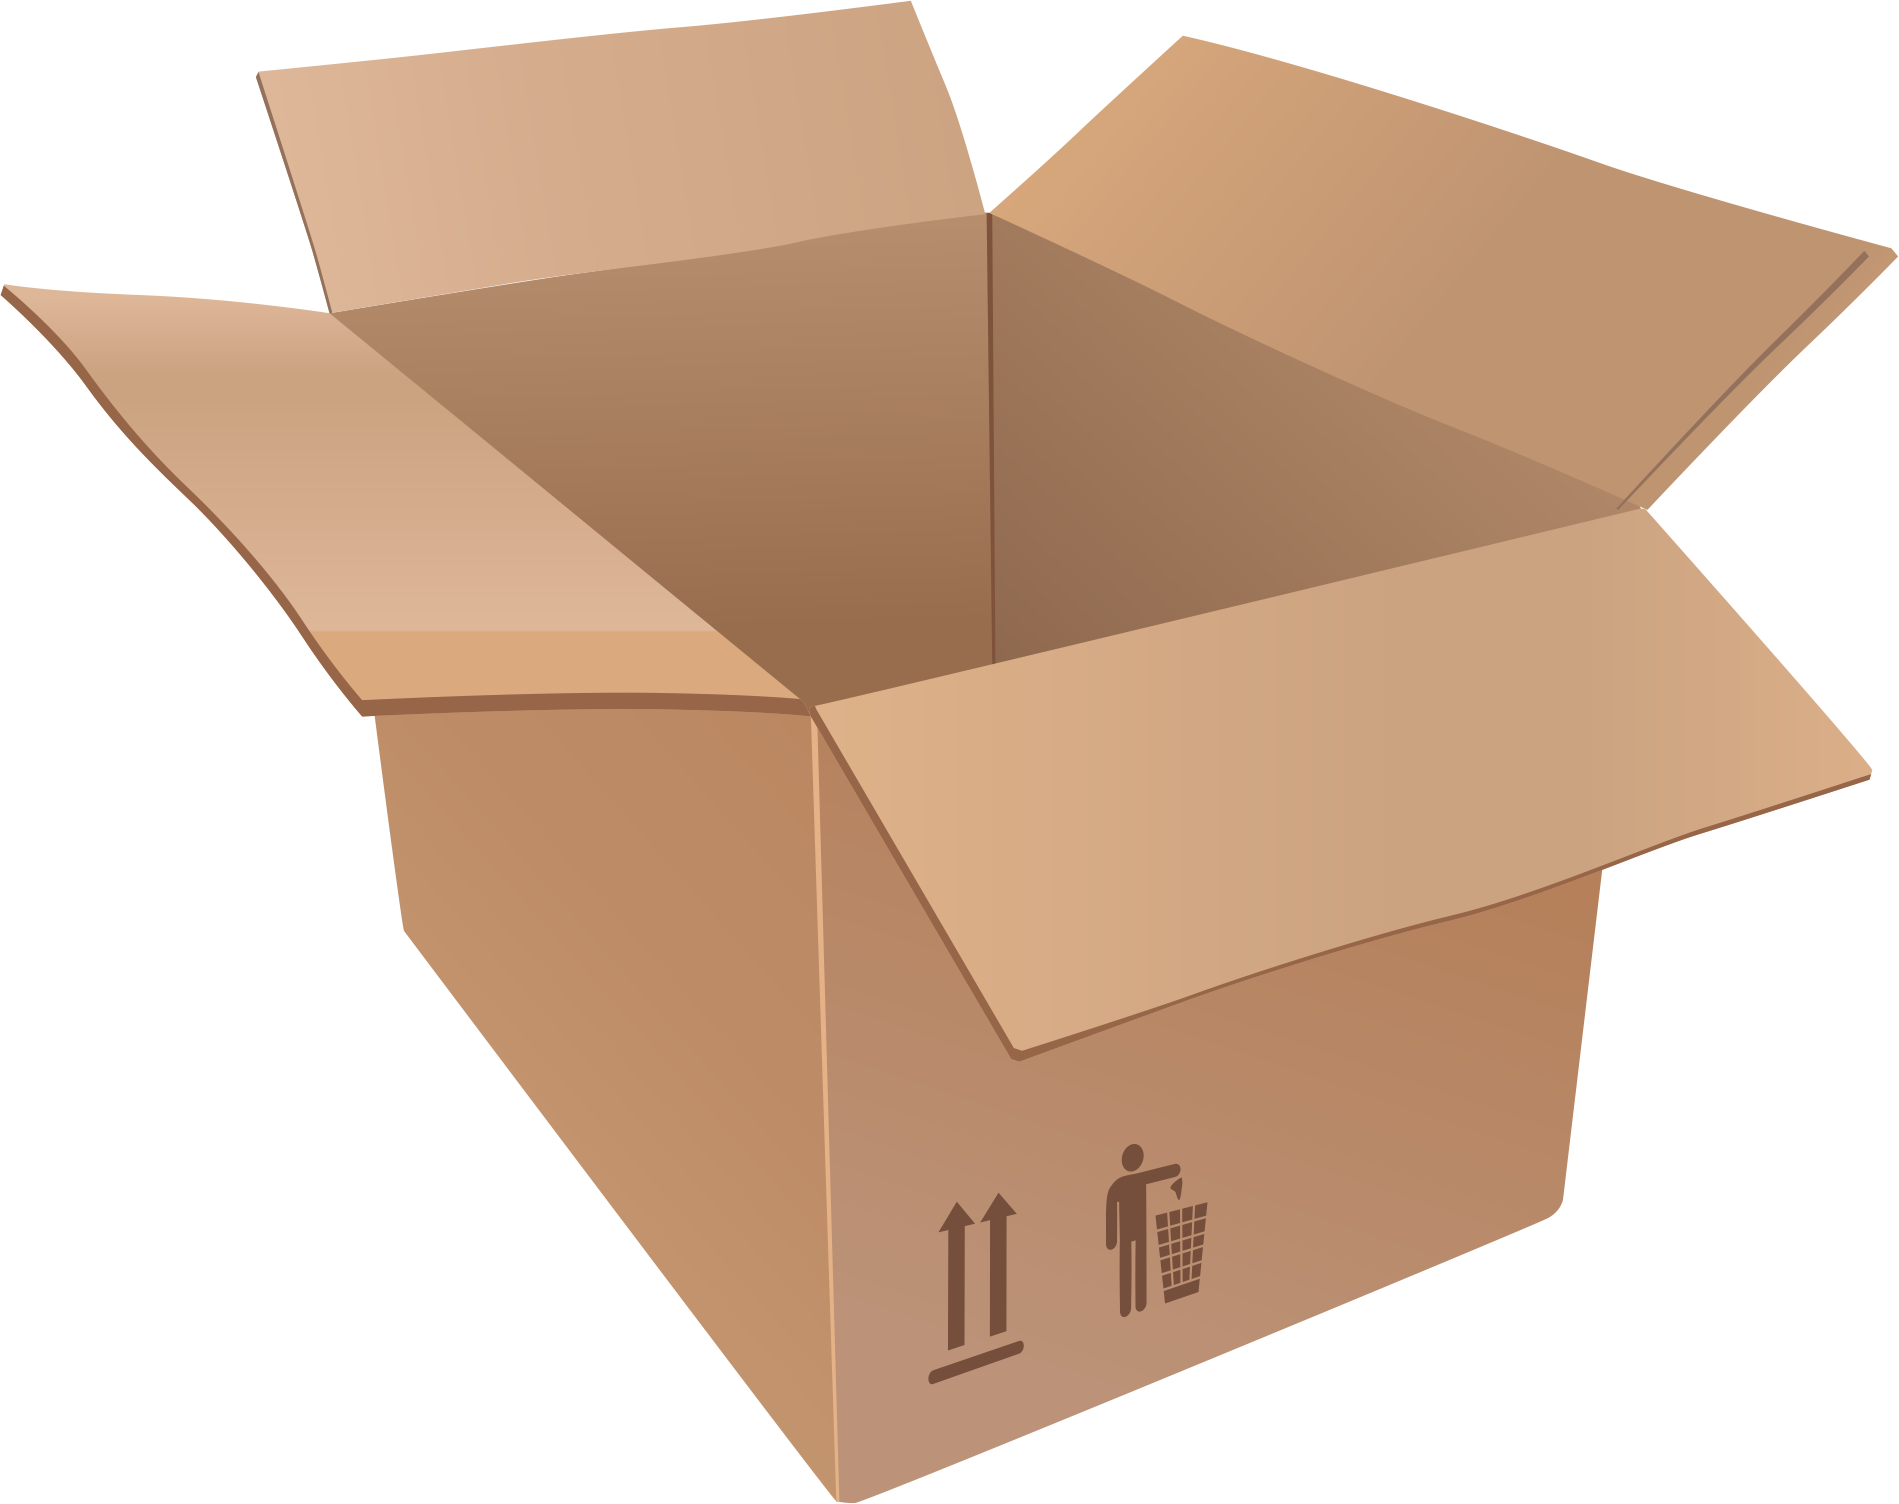
\includegraphics[height=0.4\textwidth]{Res/box}
        \note{
            Šta to Jokić može a mi ne možemo?
            Dobro, zapravo ima puno toga ali
            idalje ne može da stane u kutiju
            Kao u dosta filmova poenta predavanja
            će biti da svi mi (teoretski) imamo supermoći
        }
    \end{frame}
    \begin{frame}{Šta to pokušavamo?}
        ... iz Ideje.md
        Jokić je težak 129kg, visok 2.11m
        Kutija je standardna velicine
          ? koja je standardna velicina kutije
          - 24in x 24in x 24in gde je 1in = 2.54cm
        Nije nam bitno vreme provedeno u kutiji
        Ali kutija mora da bude potpuno zatvorena
        Pakovanje u kutiju ne sme da naskodi Jokiću
    \end{frame}
    \begin{frame}{Kretanje}
        ... iz Ideje.md
        Sta znaci da neko moze da stane u kutiju?
        Kretanjem mozemo da ga dovedemo u polozaj
        tako da se nalazi u kutiji
        Kretanje je kompozicija nekih pomeranja i rotacija
        ? Zasto <sub> ne moze da stane u kutiju?

        Kako funkcioniše kretanje u 3D
        (Rotacije, Translacije, sve moguće pomoću simetrija)
    \end{frame}
    \begin{frame}{Smeštanje}
        Međutim Jokić može da se savija :(
        \note{
            Da li neko ima ideju kako da odgovorimo na pitanje da
            li može da stane u kutiju?
        }
        (Slika zgrčenog Jokića u kutiji kako mu viri glava)
    \end{frame}
    \begin{frame}{Plivanje}
        (Jokić kako leži na vodi)
        \note{
            Kako nam je poznata masa Jokića, a znamo da (kao čovek) pluta
            na vodi možemo da procenimo njegovu zapreminu i da je uporedimo
            sa zapreminom kutije
        }
    \end{frame}
    \begin{frame}{Vozovi}
        ... Neke slike vozova
        ... Slika na kojoj se vidi zašto je put različit

    \end{frame}
    \begin{frame}{Dalja razmatranja}
        Kontrakcija dužine, dilatacija vremena...
    \end{frame}
    \begin{frame}{Cliff Hanger}
        Ako se Jokić kreće brzinom $v$ koja je blizu brzine svetlosti
        desiće se kontrakcija njegove visine i na kratko ćemo moći da
        ga smestimo u kutiju
    \end{frame}
    \begin{frame}{Da li}
        Problem?
    \end{frame}
    \begin{frame}{Jokiću trebaju naočare}
        Za Jokića je pak kutija doživela kontrakciju dužine,
        dakle u kutiju ne može da mu stane ni glava
    \end{frame}
    \begin{frame}
        Da li možemo da izdvojimo nešto fundamentalnije što bi nam
        pomoglo (kao matematičarima) da lakše razmatramo ovaj problem?
    \end{frame}
    \begin{frame}{Invarijante}
    \end{frame}
    \begin{frame}{Dalje zanimljivosti}
    \end{frame}
    \begin{frame}{Rezolujcija problema}
        slika
    \end{frame}
\end{document}
